\chapter*{Pruebas y resultados}\addcontentsline{toc}{chapter}{Pruebas y resultados}
	
	Para analizar el funcionamiento del algoritmo así como de las optimizaciones se han realizado ejecuciones de ambas versiones sobre diferentes conjuntos de reglas generados mediante FCA a partir de contextos aleatorios de diferentes tamaños. 
	
	Sobre cada conjunto de reglas se ha ejecutado el algoritmo hasta eliminar todas las variables presentes en el mismo y se ha monitorizado el tiempo de ejecución y el número de reglas resultante en cada iteración.	
	
	Para la generación de reglas se han utilizado contextos de tamaño cuadrado (mismo número de atributos que de ejemplos) que se han rellenado de forma aleatoria en base a un valor de densidad. Esta densidad representa la probabilidad de que un ejemplo posea un atributo.
	

\newpage

\section*{Resultados generales}\addcontentsline{toc}{section}{Resultados generales}

	En primer lugar analizaremos la ejecución global del algoritmo, es decir la eliminación de todas las variables. 
	
	\begin{figure}[h]
	
		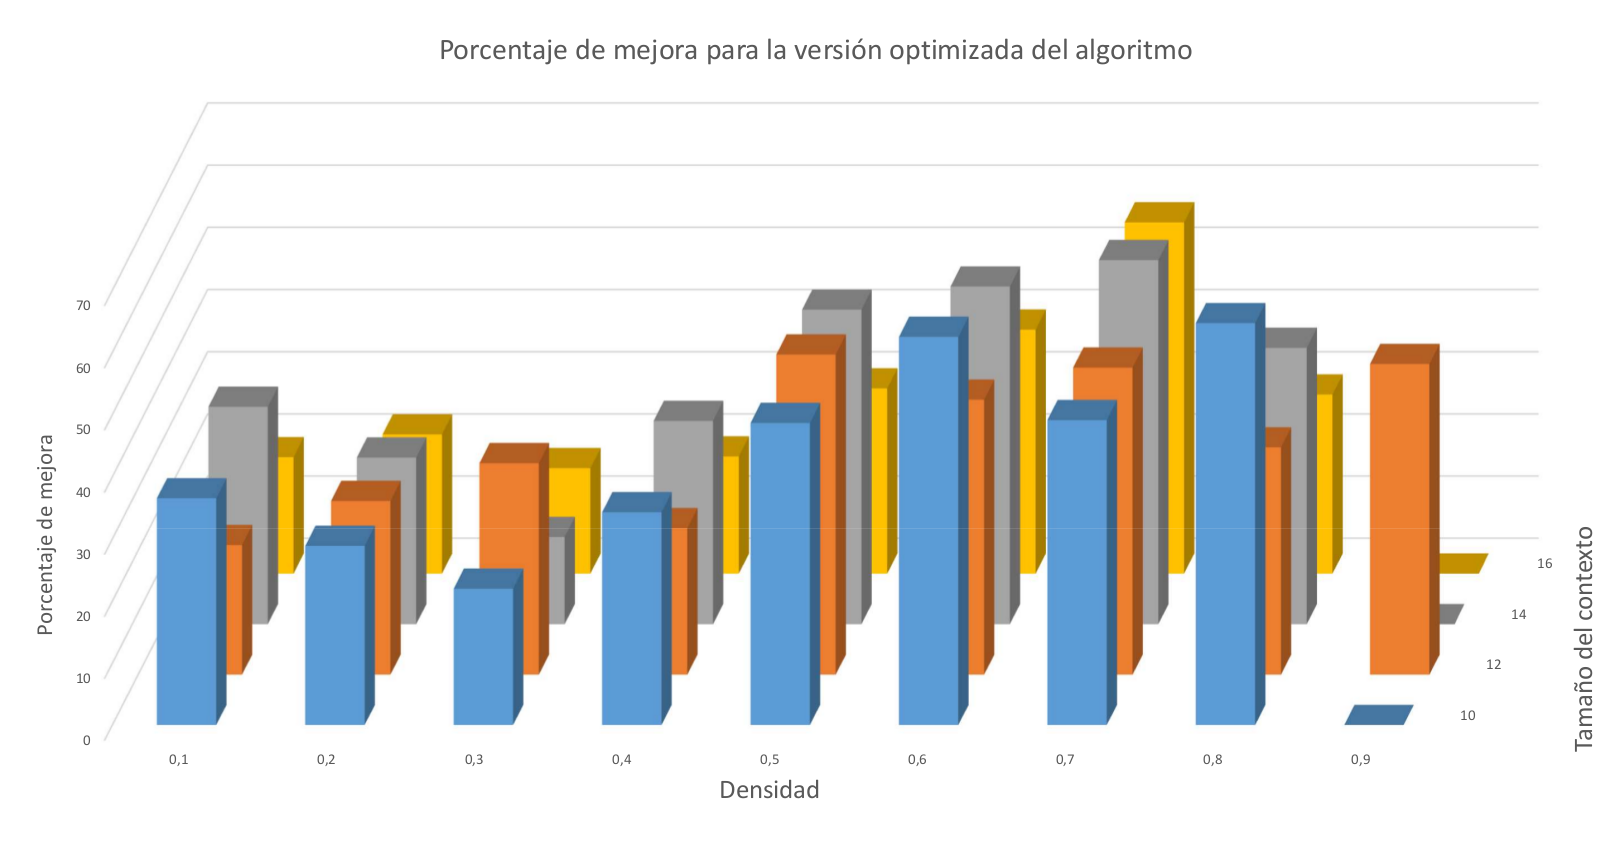
\includegraphics[width=1\linewidth]{05_Pruebas/graficas/general}
		\caption{Porcentaje de mejora del algoritmo optimizado sobre el no optimizado en función de densidad y tamaño del contexto inicial.}
		\label{fig:general}
	\end{figure}
	
	En la figura \ref{fig:general} (que representa la tabla \ref{tiempos_totales}) puede verse información de ejecuciones sobre diferentes conjuntos y el cálculo del porcentaje de mejora de la versión optimizada del algoritmo sobre la no optimizada.
	

	\begin{table}[htbp]
		\caption{Tiempos de ejecución de las dos versiones del algoritmo (v1: sin optimizaciones, v2: optimizado) para diferentes conjuntos de reglas}
		\begin{center}
			\begin{tabular}{|r|r|r|r|r|r|}
				\hline
				Tamaño Cxto & Densidad & Nº reglas & T v1 (ms) & T v2 (ms) & \% mejora \\ \hline
					\hline
				10 & 0,1 & 15 & 104 & 66 & 36,5 \\ \hline
				10 & 0,2 & 22 & 135 & 96 & 28,9 \\ \hline
				10 & 0,3 & 14 & 50 & 39 & 22,0 \\ \hline
				10 & 0,4 & 24 & 452 & 297 & 34,3 \\ \hline
				10 & 0,5 & 17 & 37 & 19 & 48,6 \\ \hline
				10 & 0,6 & 15 & 8 & 3 & 62,5 \\ \hline
				10 & 0,7 & 20 & 14 & 11 & 21,4 \\ \hline
				10 & 0,8 & 15 & 17 & 6 & 64,7 \\ \hline
				10 & 0,9 & 3 & 0 & 0 & 0 \\ \hline
				12 & 0,1 & 17 & 206 & 163 & 20,9 \\ \hline
				12 & 0,2 & 23 & 1015 & 731 & 28,0 \\ \hline
				12 & 0,3 & 31 & 734 & 484 & 34,1 \\ \hline
				12 & 0,4 & 30 & 89 & 68 & 23,6 \\ \hline
				12 & 0,5 & 49 & 1735 & 841 & 51,5 \\ \hline
				12 & 0,6 & 47 & 1130 & 630 & 44,2 \\ \hline
				12 & 0,7 & 31 & 170 & 86 & 49,4 \\ \hline
				12 & 0,8 & 35 & 82 & 52 & 36,6 \\ \hline
				12 & 0,9 & 7 & 2 & 1 & 50,0 \\ \hline
				14 & 0,1 & 41 & 16222 & 10549 & 35,0 \\ \hline
				14 & 0,2 & 36 & 9315 & 6818 & 26,8 \\ \hline
				14 & 0,3 & 77 & 682889 & 587106 & 14,0 \\ \hline
				14 & 0,4 & 81 & 121909 & 82034 & 32,7 \\ \hline
				14 & 0,5 & 56 & 3714 & 1835 & 50,6 \\ \hline
				14 & 0,6 & 68 & 6632 & 3030 & 54,3 \\ \hline
				14 & 0,7 & 95 & 9347 & 3873 & 58,6 \\ \hline
				14 & 0,8 & 39 & 135 & 75 & 44,4 \\ \hline
				14 & 0,9 & 7 & 0 & 0 & 0 \\ \hline
				16 & 0,1 & 41 & 164563 & 133748 & 18,7 \\ \hline
				16 & 0,2 & 53 & 84052 & 65228 & 22,4 \\ \hline
				16 & 0,3 & 84 & 13513731 & 11221599 & 17,0 \\ \hline
				16 & 0,4 & 110 & 3370540 & 2735275 & 18,8 \\ \hline
				16 & 0,5 & 101 & 209397 & 147008 & 29,8 \\ \hline
				16 & 0,6 & 148 & 1734667 & 1053872 & 39,2 \\ \hline
				16 & 0,7 & 80 & 3101 & 1349 & 56,5 \\ \hline
				16 & 0,8 & 53 & 243 & 173 & 28,8 \\ \hline
				16 & 0,9 & 6 & 0 & 2 & 0 \\ \hline
			\end{tabular}
		\end{center}
		\label{tiempos_totales}
	\end{table}

	En todos los casos el algoritmo con optimizaciones obtiene mejores resultados (o iguales en casos muy pequeños) que el no optimizado, variando el porcentaje de mejora \textbf{entre un 14\% y un 65\% con un valor medio de 36,5\%.}
	
	También puede observarse un mayor peso de la optimización en densidades medias-altas. Uno de los motivos a los que puede deberse esto es que a esas densidades el número resultante de reglas suele ser mayor, lo cual facilita que se creen la situaciones que las optimizaciones pueden tratar. 
	\newpage
	
\section*{Análisis por iteración}\addcontentsline{toc}{section}{Análisis por iteración}

	Ya que el objetivo del las optimizaciones implementadas es reducir el tamaño del conjunto en ejecuciones sucesivas del algoritmo, se han analizado las ejecuciones de la tabla \ref{tiempos_totales} iteración por iteración para poder ver el efecto concreto de dichas optimizaciones sobre los conjuntos de reglas.
	
	\begin{figure}[htbp]
		\centering
		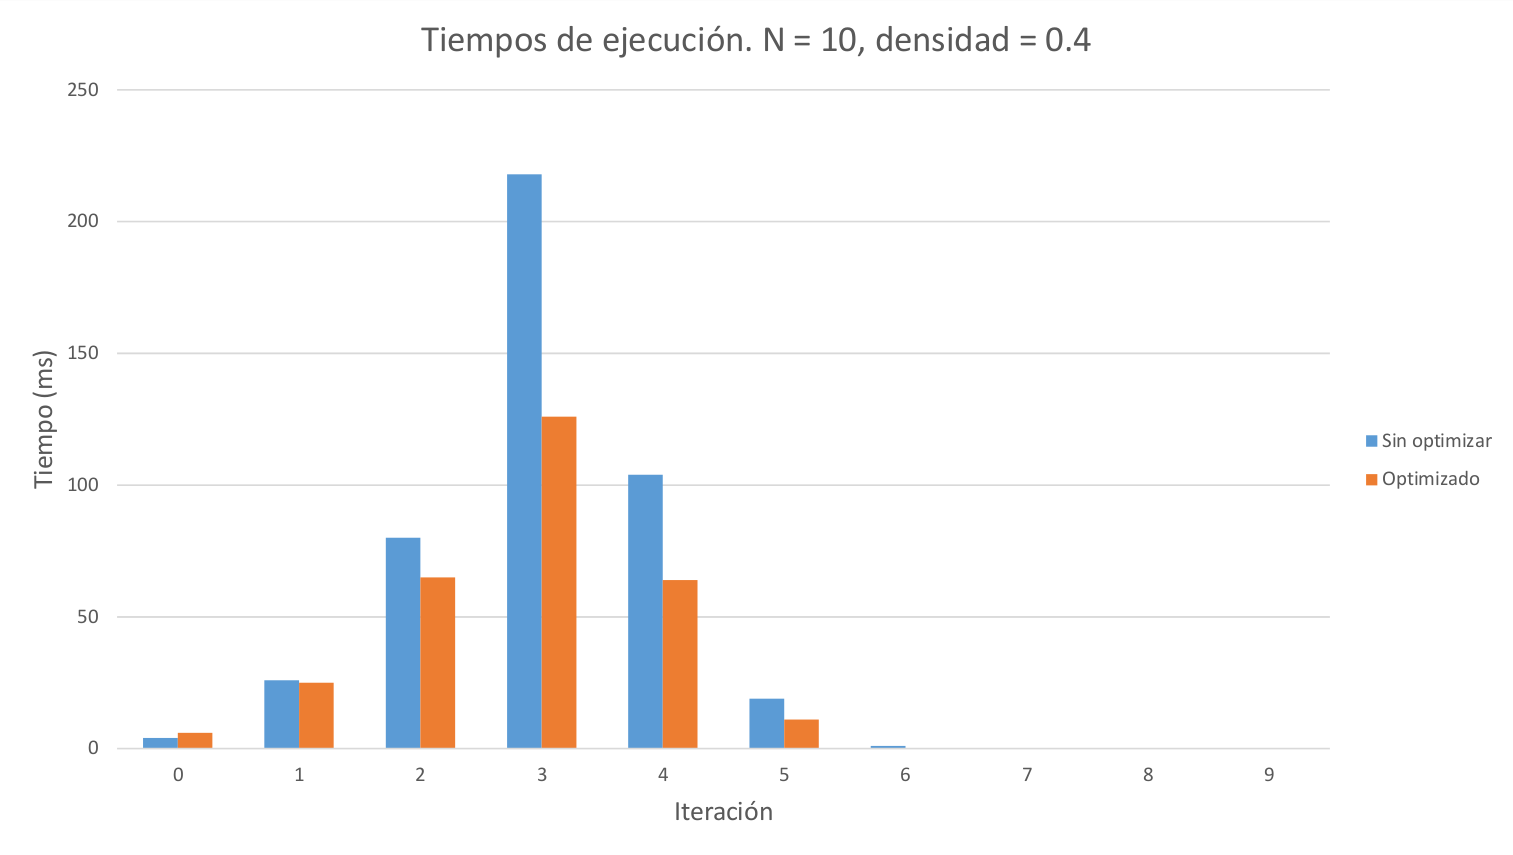
\includegraphics[width=1\linewidth]{05_Pruebas/graficas/10_4}
		\caption{Tiempos de ejecución por iteración para un contexto de tamaño 10 y densidad 0.4}
		\label{fig:10_4}
	\end{figure}

	\begin{figure}[htbp]
		\centering
		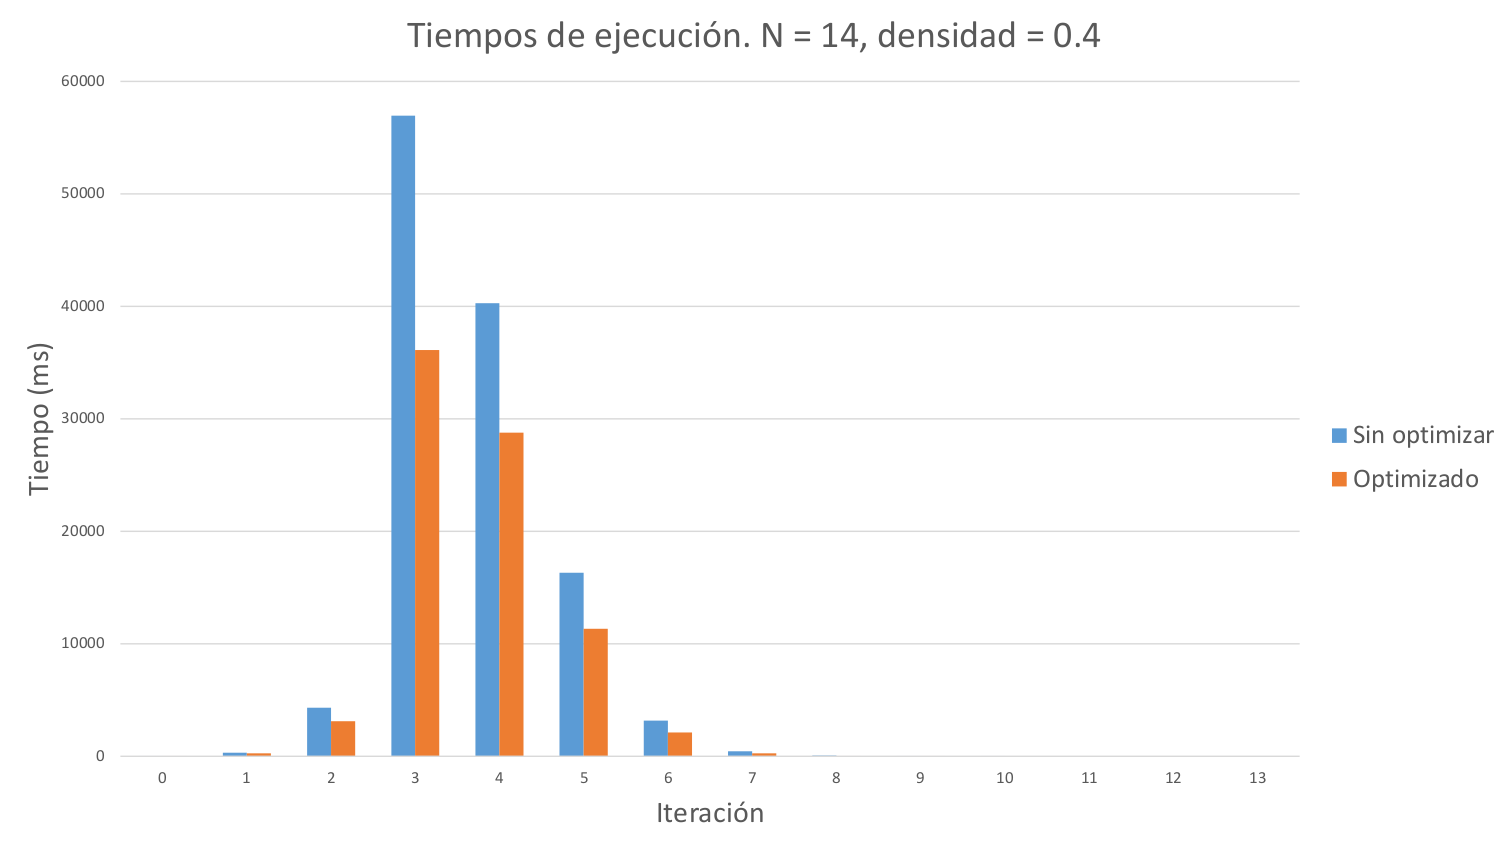
\includegraphics[width=1\linewidth]{05_Pruebas/graficas/14_4}
		\caption{Tiempos de ejecución por iteración para un contexto de tamaño 14 y densidad 0.4}
		\label{fig:14_4}
	\end{figure}
	
	\begin{figure}[htbp]
		\centering
		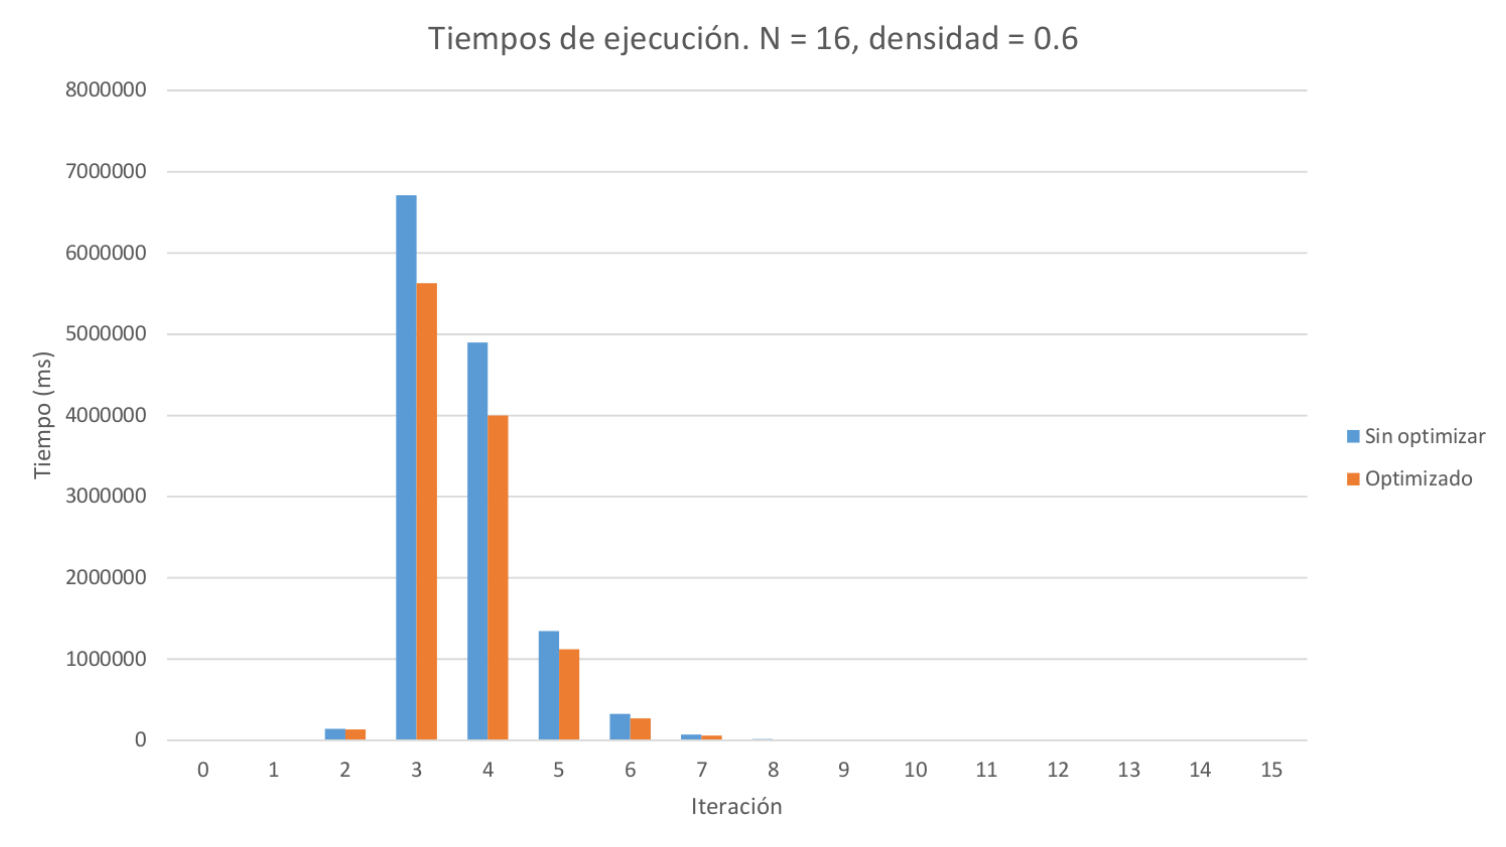
\includegraphics[width=1\linewidth]{05_Pruebas/graficas/16_3}
		\caption{Tiempos de ejecución por iteración para un contexto de tamaño 16 y densidad 0.3}
		\label{fig:16_3}
	\end{figure}
	
	En las figuras \ref{fig:10_4}, \ref{fig:14_4}, \ref{fig:16_3}  se muestran algunas de estas ejecuciones en detalle.
	
	En general, puede verse que la primera iteración presenta el mismo tiempo de ejecución para ambas versiones o en ocasiones un tiempo ligeramente mayor para la versión optimizada. Esto es lógico ya que la versión optimizada realiza más operaciones sobre el conjunto pero no se beneficia de las optimizaciones.
	
	A partir de la segunda iteración, el número de reglas del conjunto es siempre inferior en la versión optimizada, lo cual repercute en una mejora sobre los tiempos de ejecución.
	
	Estas trazas también permiten apreciar que en general el algoritmo provoca un crecimiento en el número de reglas con cada eliminación hasta que llega a un punto de inflexión tras el cual el número de reglas disminuye tras cada ejecución. 
	
	\begin{table}[htbp]
		\caption{Detalle de las iteraciones con un contexto 10x10 y densidad 0.4}
		\begin{center}
			\begin{tabular}{|r|r|r|r|r|}
				\hline 
				Iteración  & T v1 (ms) & T v2 (ms) & Tamaño Salida v1  & Tamaño Salida v2  \\ \hline \hline
				0 & 4 & 6 & 58 & 54 \\ \hline
				1 & 26 & 25 & 104 & 91 \\ \hline
				2 & 80 & 65 & 186 & 132 \\ \hline
				3 & 218 & 126 & 139 & 103 \\ \hline
				4 & 104 & 64 & 57 & 39 \\ \hline
				5 & 19 & 11 & 15 & 7 \\ \hline
				6 & 1 & 0 & 3 & 0 \\ \hline
				7 & 0 & 0 & 0 & 0 \\ \hline
				8 & 0 & 0 & 0 & 0 \\ \hline
				9 & 0 & 0 & 0 & 0 \\ \hline
			\end{tabular}
		\end{center}
		\label{iteraciones10d4}
	\end{table}


	\begin{table}[htbp]
		\caption{Detalle de las iteraciones con un contexto 14x14 y densidad 0.4}
		\begin{center}
			\begin{tabular}{|r|r|r|r|r|}
				\hline
				Iteración  & T v1 (ms) & T v2 (ms) & Tamaño Salida v1  & Tamaño Salida v2  \\ \hline \hline
				0 & 33 & 33 & 263 & 233 \\ \hline
				1 & 306 & 258 & 977 & 798 \\ \hline
				2 & 4321 & 3130 & 3858 & 2908 \\ \hline
				3 & 56965 & 36119 & 3178 & 2576 \\ \hline
				4 & 40276 & 28759 & 2092 & 1673 \\ \hline
				5 & 16315 & 11330 & 922 & 727 \\ \hline
				6 & 3171 & 2108 & 349 & 252 \\ \hline
				7 & 457 & 267 & 118 & 74 \\ \hline
				8 & 59 & 28 & 38 & 18 \\ \hline
				9 & 6 & 2 & 11 & 4 \\ \hline
				10 & 1 & 0 & 4 & 0 \\ \hline
				11 & 0 & 0 & 1 & 0 \\ \hline
				12 & 0 & 0 & 0 & 0 \\ \hline
				13 & 0 & 0 & 0 & 0 \\ \hline
			\end{tabular}
		\end{center}
		\label{iteraciones14d4}
	\end{table}
	
	\begin{table}[htbp]
		\caption{Detalle de las iteraciones con un contexto 16x16 y densidad 0.3}
		\begin{center}
			\begin{tabular}{|r|r|r|r|r|}
				\hline
				Iteración  & T v1 (ms) & T v2 (ms) & Tamaño Salida v1  & Tamaño Salida v2  \\ \hline \hline
				0 & 38 & 40 & 520 & 509 \\ \hline
				1 & 1324 & 1360 & 5611 & 5279 \\ \hline
				2 & 142854 & 135685 & 33640 & 29701 \\ \hline
				3 & 6710792 & 5628368 & 29159 & 25214 \\ \hline
				4 & 4896754 & 3996734 & 15526 & 13530 \\ \hline
				5 & 1346728 & 1119486 & 7472 & 6487 \\ \hline
				6 & 325921 & 268265 & 3625 & 3132 \\ \hline
				7 & 72416 & 58667 & 1577 & 1339 \\ \hline
				8 & 14593 & 11322 & 642 & 525 \\ \hline
				9 & 2311 & 1672 & 239 & 182 \\ \hline
				10 & 333 & 220 & 84 & 57 \\ \hline
				11 & 39 & 21 & 23 & 11 \\ \hline
				12 & 3 & 1 & 6 & 1 \\ \hline
				13 & 0 & 0 & 2 & 0 \\ \hline
				14 & 0 & 0 & 0 & 0 \\ \hline
				15 & 1 & 0 & 0 & 0 \\ \hline
			\end{tabular}
		\end{center}
		\label{iteraciones16d3}
	\end{table}
	
		

\section*{Comparación entre generación y retracción}\addcontentsline{toc}{section}{Comparación entre generación y retracción}		
		
	Por último se ha comparado el tiempo necesario para generar las implicaciones correspondientes a un contexto de tamaño N y el tiempo necesario para obtener un conjunto de implicaciones equivalente a partir de un contexto de tamaño N+1.
	
	Para contextos de tamaño menor a 30 generar el contexto es más rápido que calcular la retracción conservativa sobre un conjunto generado a partir de un contexto con una variable adicional.
	
	Sin embargo para tamaños mayores el tiempo se iguala y finalmente a partir de tamaño 36 (como puede verse en la figura \ref{generacion}) resulta más rápido calcular la retracción que generar el conjunto desde cero.
	
	
	\begin{figure}[h]
		\centering
		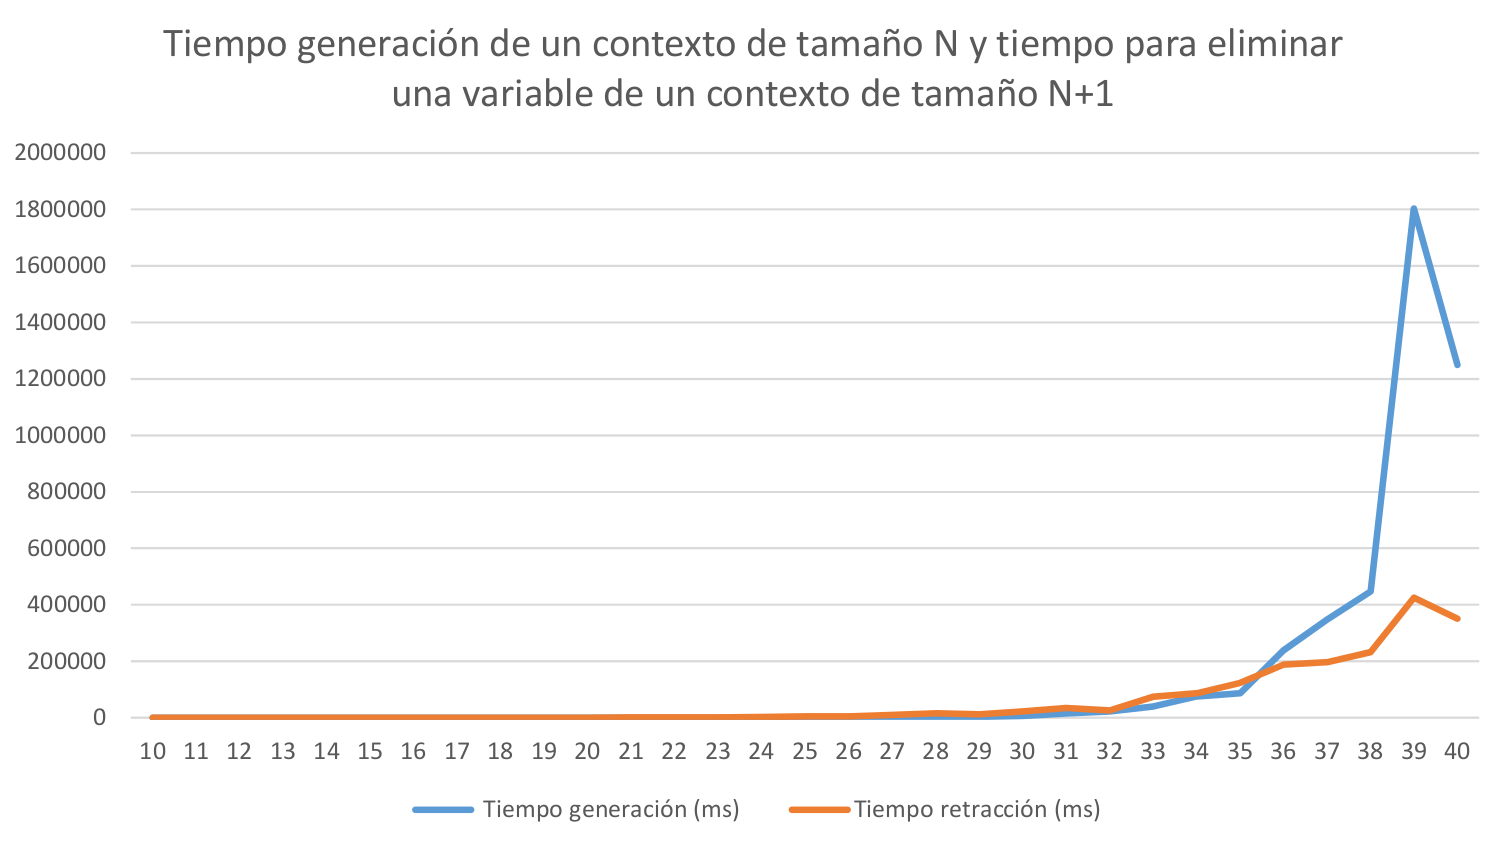
\includegraphics[width=1\linewidth]{05_Pruebas/graficas/generacionLineas}
		\caption{Tiempos de generación y retracción de conjuntos del mismo tamaño}
		\label{generacion}
	\end{figure}

		